\documentclass[]{elsarticle} %review=doublespace preprint=single 5p=2 column
%%% Begin My package additions %%%%%%%%%%%%%%%%%%%
\usepackage[hyphens]{url}

  \journal{European Economic Review} % Sets Journal name


\usepackage{lineno} % add

\usepackage{graphicx}
%%%%%%%%%%%%%%%% end my additions to header

\usepackage[T1]{fontenc}
\usepackage{lmodern}
\usepackage{amssymb,amsmath}
\usepackage{ifxetex,ifluatex}
\usepackage{fixltx2e} % provides \textsubscript
% use upquote if available, for straight quotes in verbatim environments
\IfFileExists{upquote.sty}{\usepackage{upquote}}{}
\ifnum 0\ifxetex 1\fi\ifluatex 1\fi=0 % if pdftex
  \usepackage[utf8]{inputenc}
\else % if luatex or xelatex
  \usepackage{fontspec}
  \ifxetex
    \usepackage{xltxtra,xunicode}
  \fi
  \defaultfontfeatures{Mapping=tex-text,Scale=MatchLowercase}
  \newcommand{\euro}{€}
\fi
% use microtype if available
\IfFileExists{microtype.sty}{\usepackage{microtype}}{}
\bibliographystyle{elsarticle-harv}
\ifxetex
  \usepackage[setpagesize=false, % page size defined by xetex
              unicode=false, % unicode breaks when used with xetex
              xetex]{hyperref}
\else
  \usepackage[unicode=true]{hyperref}
\fi
\hypersetup{breaklinks=true,
            bookmarks=true,
            pdfauthor={},
            pdftitle={An Independent European Macro? A History of European Macroeconomics through the Lens of the European Economic Review},
            colorlinks=false,
            urlcolor=blue,
            linkcolor=magenta,
            pdfborder={0 0 0}}
\urlstyle{same}  % don't use monospace font for urls

\setcounter{secnumdepth}{5}
% Pandoc toggle for numbering sections (defaults to be off)


% tightlist command for lists without linebreak
\providecommand{\tightlist}{%
  \setlength{\itemsep}{0pt}\setlength{\parskip}{0pt}}


% Pandoc citation processing
\newlength{\cslhangindent}
\setlength{\cslhangindent}{1.5em}
\newlength{\csllabelwidth}
\setlength{\csllabelwidth}{3em}
\newlength{\cslentryspacingunit} % times entry-spacing
\setlength{\cslentryspacingunit}{\parskip}
% for Pandoc 2.8 to 2.10.1
\newenvironment{cslreferences}%
  {}%
  {\par}
% For Pandoc 2.11+
\newenvironment{CSLReferences}[2] % #1 hanging-ident, #2 entry spacing
 {% don't indent paragraphs
  \setlength{\parindent}{0pt}
  % turn on hanging indent if param 1 is 1
  \ifodd #1
  \let\oldpar\par
  \def\par{\hangindent=\cslhangindent\oldpar}
  \fi
  % set entry spacing
  \setlength{\parskip}{#2\cslentryspacingunit}
 }%
 {}
\usepackage{calc}
\newcommand{\CSLBlock}[1]{#1\hfill\break}
\newcommand{\CSLLeftMargin}[1]{\parbox[t]{\csllabelwidth}{#1}}
\newcommand{\CSLRightInline}[1]{\parbox[t]{\linewidth - \csllabelwidth}{#1}\break}
\newcommand{\CSLIndent}[1]{\hspace{\cslhangindent}#1}

\usepackage{float}
\usepackage{booktabs}
\usepackage{longtable}
\usepackage{array}
\usepackage{multirow}
\usepackage{wrapfig}
\usepackage{colortbl}
\usepackage{pdflscape}
\usepackage{tabu}
\usepackage{threeparttable}
\usepackage{threeparttablex}
\usepackage[normalem]{ulem}
\usepackage{makecell}
\usepackage{xcolor}



\begin{document}


\begin{frontmatter}

  \title{An Independent European Macro? A History of European
Macroeconomics through the Lens of the European Economic Review}
    \author[1]{Aurélien Goutsmedt\corref{3}}
  
    \author[2]{Alexandre Truc}
  
      \address[1]{UCLouvain, ISPOLE. Collège Jacques Leclercq, Place
Montesquieu, 1/L 2.08.07, 1348 - Louvain-la-Neuve.}
    \address[2]{Université Côte d'Azur, CNRS GREDEG France.}
      \cortext[3]{Corresponding Author: aurelien.goutsmedt@uclouvain.be}
  
  \begin{abstract}
  Economics in Europe has encountered a process of internationalisation
  since the 1970s. To a certain extent, this internationalisation is
  also an `Americanisation' and many European departments and economics
  have adopted the standards of US economics, notably mathematical
  modelling, the use of econometrics, and the neoclassical theory as a
  modelling benchmark. Regarding this process, we can wonder if European
  economics has just been mimicking US economics since the 1970s, or if
  some European specialities have survived or emerged.

  In this article, we use topic modelling and bibliometric coupling to
  identify what have been some European specialities between 1969 and
  2002. We focus on one economics sub-discipline, macroeconomics, and we
  use the articles published in the European Economic Review and compare
  their bibliographic references and content to what has been published
  in the top 5 journals.
  \end{abstract}
  
 \end{frontmatter}

\hypertarget{introduction}{%
\section{Introduction}\label{introduction}}

In 1987, the then director of the Centre for Economic Policy Research,
Richard Portes, attempted to assess the ``state and status of economics
in Europe'' in the \emph{European Economic Review}. He regarded ``the
standard of comparison {[}as{]} obvious: the United States, by far the
dominant producer'' (\protect\hyperlink{ref-portes1987}{Portes, 1987, p.
1329}). He thus asked ``whether there is now any economics outside and
independent of the United States.'' (1330) He gave a list of the many
indices testifying of the US domination, ending it by the fact that
``the leaders of the economics profession in Europe were trained as
postgraduates in the United States. Many take from the US their
professional standards, their views of what are the interesting
problems, and their approaches to them''. (\emph{ibid.})

Indeed, since the early 1970s, economics in many Western European
countries had entered in a process of internationalisation
(\protect\hyperlink{ref-fourcade2009}{Fourcade, 2009, chap. 3} and 4;
\protect\hyperlink{ref-fourcade2006}{Fourcade, 2006}). On a large
extent, such process was also a form of ``Americanisation''
(\protect\hyperlink{ref-coats1996}{Coats, 1996};
\protect\hyperlink{ref-goutsmedt2021}{Goutsmedt et al., 2021}):
professional and intellectual standards were progressively adopted in
European countries, mimicking the functioning of the US academic field.
English gradually spread as the dominant language in economics
(\protect\hyperlink{ref-sandelin1997}{Sandelin and Ranki, 1997}) and
publications in peer-review journals became the norm for assessing
research productivity. The organisation of international events were
encouraged to boost research centres visibility
(\protect\hyperlink{ref-goutsmedt2021}{Goutsmedt et al., 2021}). In
terms of content, the Americanisation of the discipline in Europe
favoured the intellectual standards that had become widespread in the US
in the postwar era (\protect\hyperlink{ref-morgan1998}{Morgan and
Rutherford, 1998}): the use of mathematical economics and econometrics,
and the reliance on neoclassical theory as a benchmark for
modelling.\footnote{Of course, this process of Americanisation did not
  go without conflicts: many ``local conflicts'' emerged between more
  ``nationally-trained'' economists (generally locally trained) and
  ``internationally-trained economists'' who had been often trained in
  the US (\protect\hyperlink{ref-fourcade2006}{Fourcade, 2006}). These
  conflicts involved intellectual matters (for instance around the
  relevance of the neoclassical theory) as well as institutional issues,
  like the criteria to assess the quality of economists' work and thus
  to determine hiring and promotion.}

In parallel to this Americanisation, we can observe a process of
`Europeanisation': many initiatives from the creation of the
\emph{European Economic Review} (EER)in 1969 to the creation of the
\emph{Economic European Association} (EEA) in 1984 promoted the
development of intellectual exchanges between European
economists---while obviously keeping US economics as a model. The
simultaneous spreading of US standards in Europe after the 1970s and the
promotion of a European economics transcending national traditions bring
us back to Portes's 1987 question: was there a possibility after the
1970s for the existence of a European tradition of economics, relatively
autonomous from the US profession?

Portes distinguished European ``comparative advantages''
(\protect\hyperlink{ref-portes1987}{Portes, 1987, p. 1332}) even if some
of these European specialities had been pioneered by US economics. He
highlighted the dynamism in Europe of ``general equilibrium
theory{[},{]} social choice, duality, and the analysis of repeated
games'', ``international macroeconomic policy coordination'' or
``Non-Walrasian macroeconomics'' (\emph{ibid}.).
(\protect\hyperlink{ref-goutsmedt2021}{Goutsmedt et al., 2021}) have
also highlighted that within the \emph{International Seminar on
Macroeconomics} (ISoM), whose proceedings were published annually in the
EER, disequilibrium or Non-Walrasian macroeconomics and large-scale
macroeconometric modelling constituted important rallying points until
the mid-1980s for the European economists involved in the ISoM.

The purpose of our article is to investigate this issue systematically
and quantitatively. Regarding the history of the EER and its importance
in the promotion of a European economics (see section
\ref{EER-creation}), we think that it constitutes a good proxy for
observing the emergence of `European specialities'. We define as
widespread research topics \emph{(i)} distinct from what US-based
economists were doing, \emph{(ii)} adopted by many European-based
economists in different European countries, and \emph{(iii)} bringing
collaboration between different universities. Using bibliometric
coupling and topic modelling joined to qualitative content analysis, we
identify European specialities from 1973 to 2002 (section
\ref{european-specialities}).\footnote{{[}Could be revised depending on
  our final choices{]} The corpus we use (see section \ref{methods}) has
  very few abstracts between 1969 (the date of the creation of the EER)
  and 1972. Besides, there is no JEL code for EER articles before 1973,
  preventing us for identifying macroeconomics articles. After 2002 and
  the creation of the \href{https://academic.oup.com/jeea}{\emph{Journal
  of the European Economic Association}}\emph{,} the EER was not the
  official journal of the EEA any more.}

The history of recent economics has mimicked the hierarchy of the
discipline by focusing mainly on US economists (and their ideas) or
institutions. Of course, some history of economics articles have dealt
with the peculiarities of economics in some European countries since the
1970s or with important European economists
(\protect\hyperlink{ref-benest2019}{Benest, 2019};
\protect\hyperlink{ref-maes2005}{Maes and Buyst, 2005}). However, our
goal here is to investigate this issue at the European level and to
understand if the internationalisation of the discipline since the 1970s
have been accompanied by the emergence of European specialities,
relatively independent of the US main topics and overcoming mere
national traditions. Besides, we use quantitative methods, as we think
that the latter are useful to get a general picture while limiting
biased choices and focus.\footnote{Indeed, it could be easy and tempting
  to pick such or such areas of study and find one or two important
  European economists working on it, to make it a European speciality.
  Even if they involve choices and interpretations, we think that the
  methods we use limit this risk}

However, we are focusing only on macroeconomics articles, mainly because
we think that such an investigation involved in-depth qualitative
\emph{and} qualitative analyses of these specialities and a relatively
good knowledge of the literature. A similar investigation on the whole
economic field would have been beyond our analytical capabilities.
Besides, macroeconomics constituted a substantial part of EER
publications, even representing almost half of all the articles in the
early 1980s (Figure \ref{fig:plot-jel}). Macroeconomics was also
instrumental in fostering collaborations between European economists as
the ``International Seminar on Macroeconomics'' testifies (see Section
\ref{rising-journal}). This article also relies on a unique dataset,
which has been constituted by merging the content of four different
institutional databases (see Section \ref{methods}).\footnote{The
  article is also accompanied by a detailed methodological
  \protect\hyperlink{appendix}{Appendix}.}

\begin{figure}[h]

{\centering \includegraphics[width=1\linewidth]{C:/Users/goutsmedt/Mon Drive/data/EER/pictures/Graphs/mean_jel} 

}

\caption{Share of Articles with at least one macroeconomics JEL code}\label{fig:plot-jel}
\end{figure}

\hypertarget{EER-creation}{%
\section{The Creation of the EER}\label{EER-creation}}

\hypertarget{a-european-project-with-us-influence}{%
\subsection{A European project with US
influence}\label{a-european-project-with-us-influence}}

In 1969, Jean Waelbroeck and Herbert Glejser, both from the
\emph{Université Libre de Bruxelles} (ULB), launched the \emph{European
Economic Review}. The new review was planned to be the official journal
of the European Scientific Association of Applied Economics (ASEPELT),
which had been created in 1961 by Waelbroeck and another ULB economist:
Etienne Kirschen. Before 1969, the association published in English a
bulletin gathering research in econometrics and mathematical economics
(\protect\hyperlink{ref-waelbroeck1969}{Waelbroeck and Glejser, 1969, p.
4}). The EER took up this torch by advertising and publishing the same
type of research. Articles in the EER had to be published in English,
the new ``\emph{lingua franca} of economics'' triggering the process of
``internationalisation of our science'' as Waelbroeck and Glejser
polemically stated in the introduction of the first issue
(\emph{ibid.}).

The fact that such a project was born in Belgium is not a coincidence.
Indeed, the country displayed a high effervescence regarding the
internationalization of the discipline. In 1966, Jacques Drèze
established the Center for Operations Research and Econometrics (CORE)
at the \emph{Katholieke Universiteit Leuven} (before its split), on the
model of the Cowles Commission and the Carnegie Institute of Technology,
which Drèze had visited in the 1950s
(\protect\hyperlink{ref-duppe2017}{Düppe, 2017}).\footnote{KU Leuven was
  split in 1968 between a Flamish and a French-speaking part, the latter
  giving birth to the \emph{Université Catholique de Louvain} at
  Louvain-La-Neuve, where the CORE eventually moved in the mid-1970s.}
The CORE developed a research program around econometrics and
macroeconomic modelling and quickly stimulated the establishment of a
European research network of economists, notably through its large
visiting programme (\protect\hyperlink{ref-duppe2017}{Düppe, 2017};
\protect\hyperlink{ref-maes2005}{Maes and Buyst, 2005}). Encouraged by
Waelbroeck, the ULB department of economics joined the CORE in its first
years of existence (\protect\hyperlink{ref-maes2005}{Maes and Buyst,
2005, p. 79}).

This context made of the EER a Belgian-centred initiative in the first
years. Belgian institutions represented one fourth of authors'
affiliations in EER articles in the first years (Figure
\ref{fig:plot-authors}).\footnote{This is an approximation, as the
  affiliation per author is not available in our corpus and we only have
  the affiliations per article (see
  \protect\hyperlink{author-affiliation}{Appendix B.2.} for more
  details).} Nonetheless, the EER authorship became increasingly diverse
in the 1970s in terms of geographic affiliation. We observe the same for
the editorial boards that, from the beginning, displayed an equilibrium
between several Western European countries (Figure
\ref{fig:plot-boards}).

\begin{figure}[h]

{\centering \includegraphics[width=1\linewidth]{C:/Users/goutsmedt/Mon Drive/data/EER/pictures/Graphs/EER_affiliations} 

}

\caption{Share of countries of authors' affiliations in EER publications (Top 10)}\label{fig:plot-authors}
\end{figure}

The EER was one of these important initiatives that contributed to the
development of intellectual exchanges between European based economists
(\protect\hyperlink{ref-goutsmedt2021}{Goutsmedt et al., 2021}). The
centrality of the journal was strengthened in 1984 when the European
Economic Association was created, and the EER established as the
official journal of the new association.

\begin{figure}[h]

{\centering \includegraphics[width=1\linewidth]{C:/Users/goutsmedt/Mon Drive/data/EER/pictures/Graphs/Board_affiliations} 

}

\caption{Share of countries in EER editorial boards (Top 10)}\label{fig:plot-boards}
\end{figure}

\hypertarget{rising-journal}{%
\subsection{A Rising European Journal}\label{rising-journal}}

Outside of offering a common platform for European economists, the
journal initial goal was also to encourage the promotion of a US style
of doing economics. An important dimension of the journal was thus the
progressive integration of US-based economists. The ``International
Seminar on Macroeconomics,'' co-organized by the French \emph{Ecole des
Hautes Etudes en Sciences Sociales} and the US National Bureau of
Economic Research, played a key role in that integration of US
economists, as the conference papers were published each year in a
special issue. It also likely contributed to make the journal known on
the other side of the Atlantic.

The share of US-based authors publishing in the journal grew steadily in
the 1970s and reached a third of all affiliations in the early 1980s
(Figure \ref{fig:plot-authors}). The increase of US economists
participation to the EER does not mean uniquely that more articles were
published by US authors, but also that number of collaborations between
US- and European-based economists increased (Figure
\ref{fig:plot-collabs}). While there was no collaboration in the first
year of the journal, 10 percent of the articles published in 1980 mixed
institutions from the US and Europe.

\begin{figure}[h]

{\centering \includegraphics[width=1\linewidth]{C:/Users/goutsmedt/Mon Drive/data/EER/pictures/Graphs/EER_collab_stack_density} 

}

\caption{Patterns of collaboration between the United States and European countries in EER}\label{fig:plot-collabs}
\end{figure}

\begin{figure}[h]

{\centering \includegraphics[width=1\linewidth]{C:/Users/goutsmedt/Mon Drive/data/EER/pictures/Graphs/Collab_strict} 

}

\caption{Patterns of collaboration between the United States and European countries in EER (noodle version)}\label{fig:plot-collabs2}
\end{figure}

In the mid-1980s, the journal was thus a symbol of a more integrated
European economics, inspired by the US standards, as well as it was
attracting many US economists to publish in it. Its intellectual
influence similarly expanded and it became a major economic journal,
overcoming other important European journals in terms of bibliographic
citations (Figure \ref{fig:plot-eer-importance}).

\begin{figure}[h]

{\centering 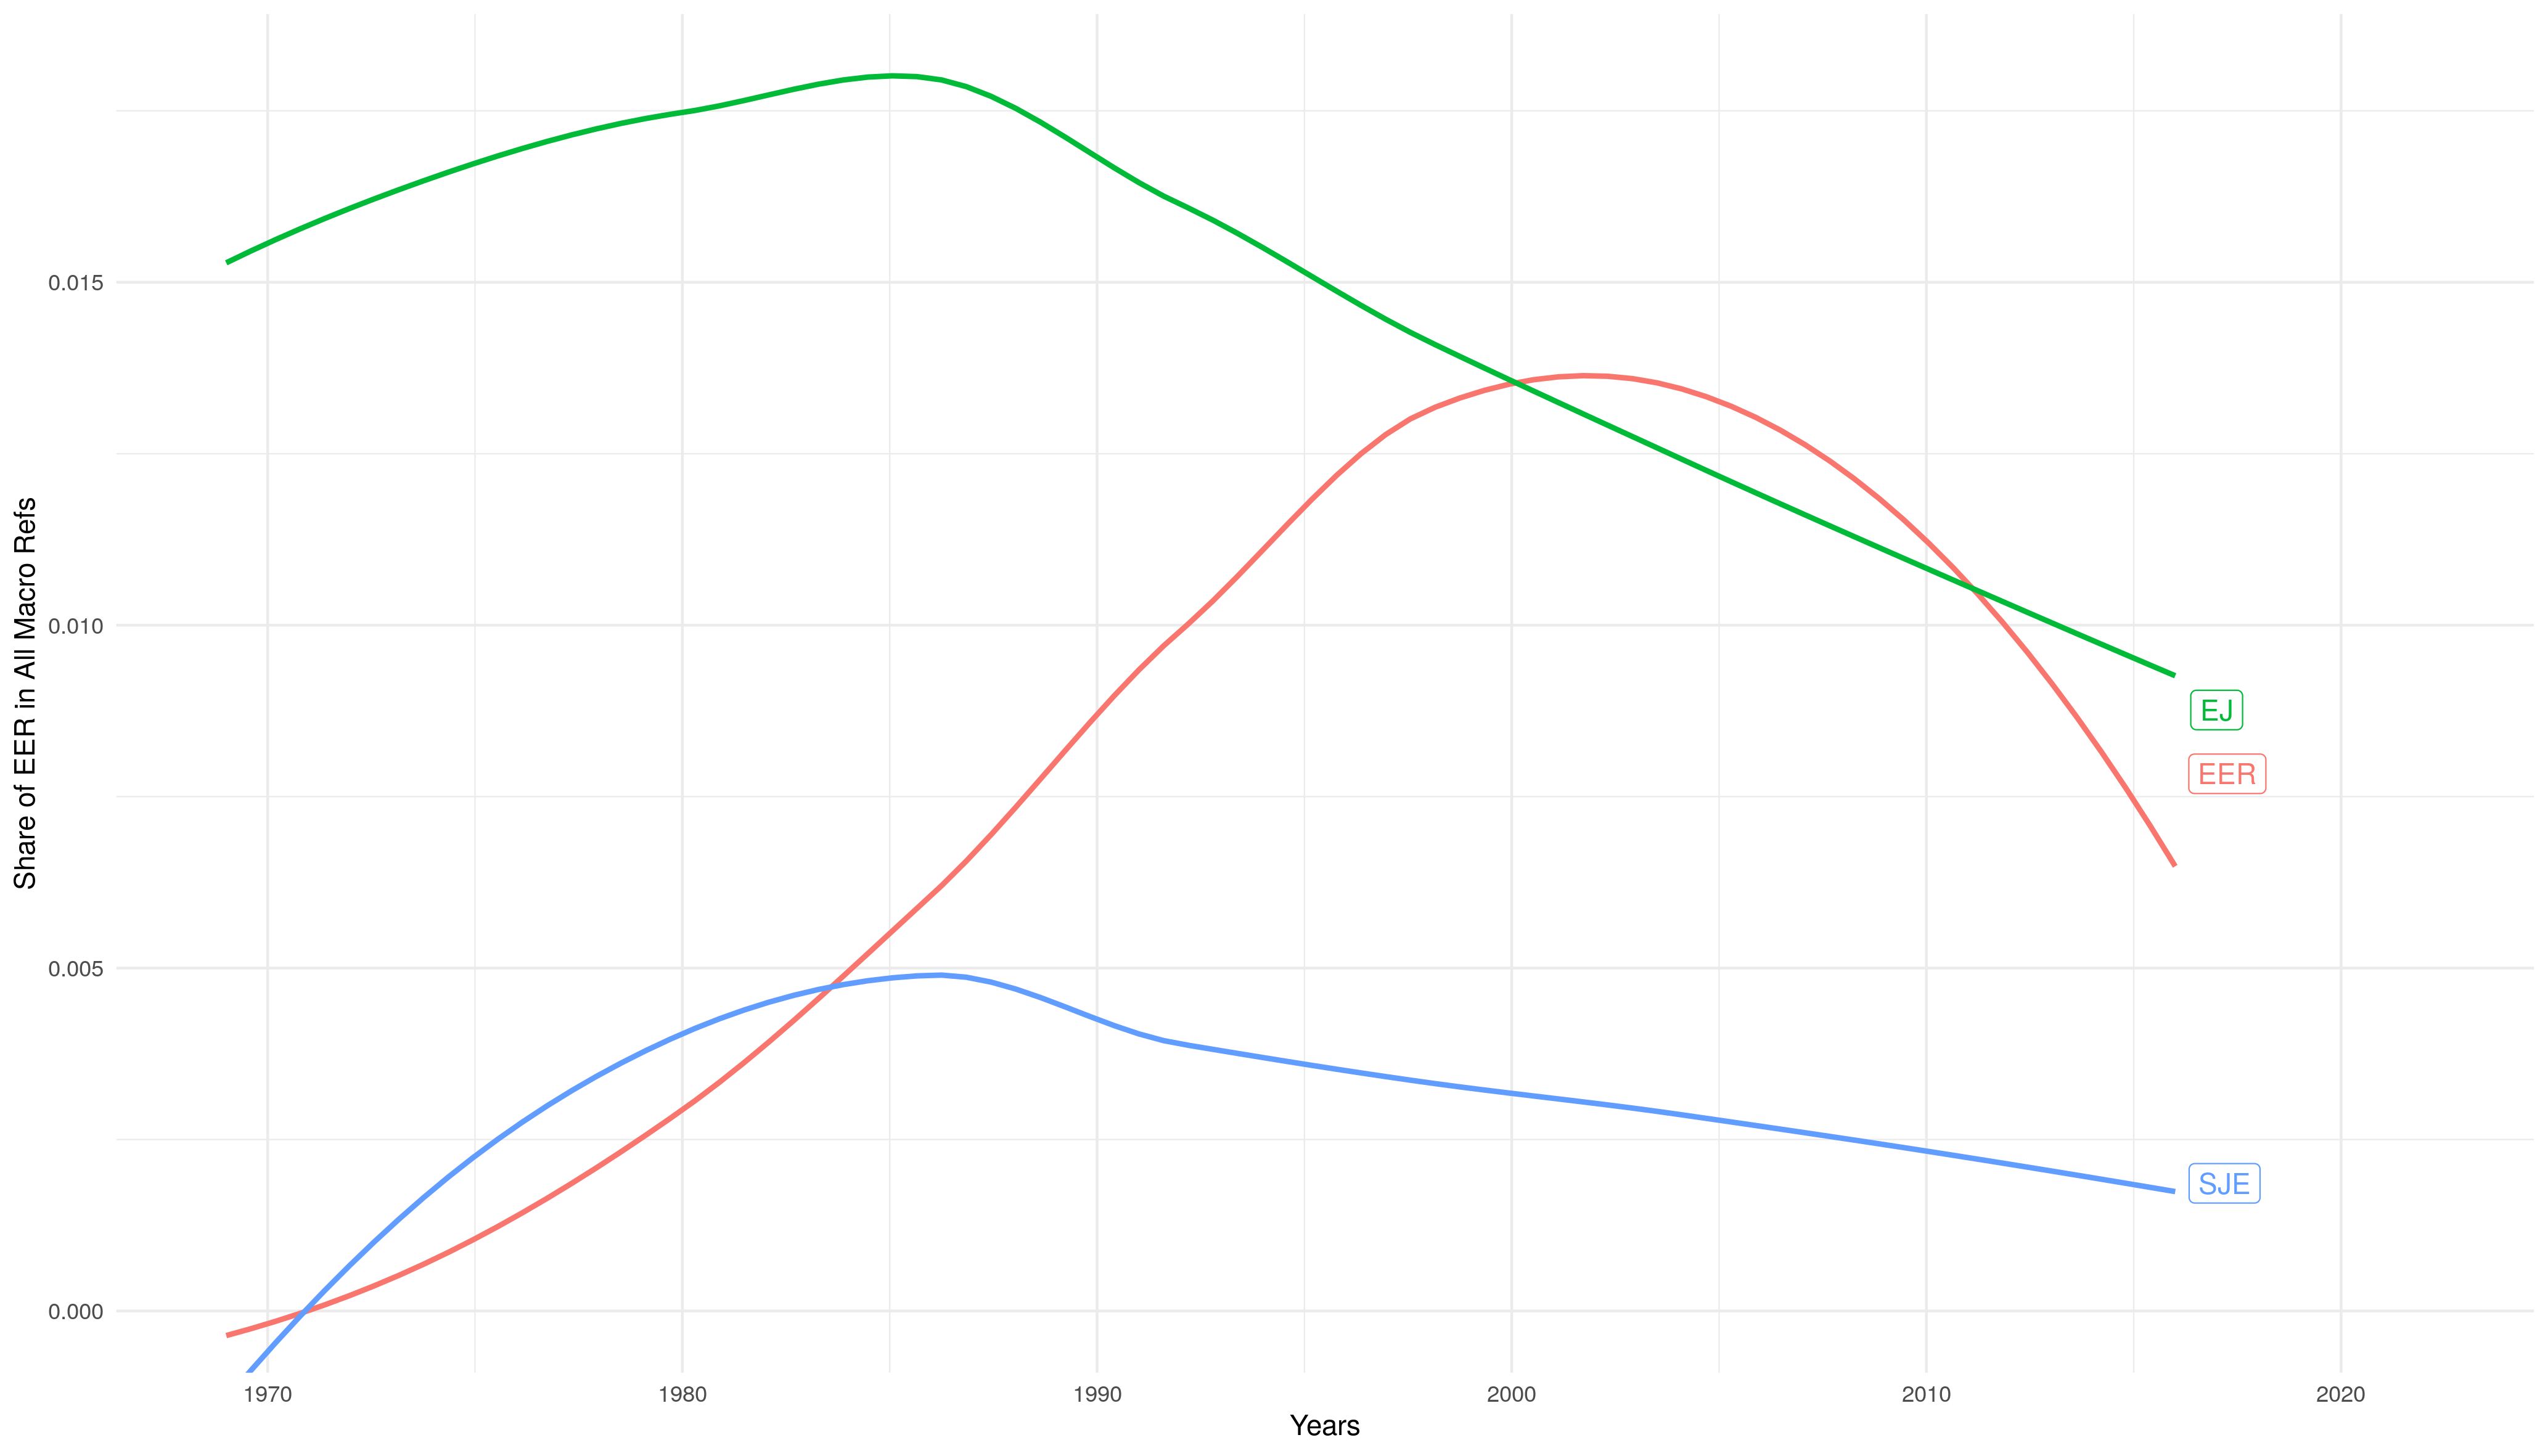
\includegraphics[width=1\linewidth]{C:/Users/goutsmedt/Mon Drive/data/EER/pictures/Graphs/EER_Importance} 

}

\caption{Share of total citations going to EER}\label{fig:plot-eer-importance}
\end{figure}

But has this whole process led to the total standardisation of a
European economics on the US model, or has it led to the development (or
persistence) of proper European specialities?

\hypertarget{european-specialities}{%
\section{Identifying European
Specialities}\label{european-specialities}}

The first step was to build our dataset. To identify European
specialities, we compare macroeconomics articles published in EER and in
the Top-5 journals, that is the \emph{American Economic Review}, the
\emph{Journal of Political Economy}, \emph{Econometrica}, the
\emph{Quarterly Journal of Economics} and the \emph{Review of Economic
Studies}. Focusing on the Top 5 allows us to only get the most popular
and dominant trends in macroeconomics and thus to draw clearer
comparisons with what is published in the EER. Besides, the EER was
created with the intent to establish an elite leading journal for the
European community that would imitate the standards of US major journal.
The Top 5 journals thus seem an adequate benchmark to compare the EER
to.

We identify macroeconomics articles by using the former and new JEL code
classification (\protect\hyperlink{ref-jel1991}{JEL, 1991}).\footnote{See
  the complete list of all the JEL codes we have used in
  \protect\hyperlink{eer-top5-macro}{Appendix B.1.}.} Outside of JEL
codes data, we have used three different databases to collect different
types of information: outside of basic metadata (year of publication,
title, authors, \emph{etc.}), we have collected the list of
bibliographic references of EER and Top-5 articles, the abstracts, and
authors affiliations.\footnote{Crossing databases has been necessary due
  to missing years and information in the different databases we have
  used (Web of Science, Scopus and Microsoft Academic Premier). See the
  \protect\hyperlink{corpus}{Appendix B.1.} for more details on the
  building of our dataset.} Then, we have conducted two different types
of analysis to identify European specialities.

\hypertarget{bibliographic-coupling}{%
\subsection{Bibliographic coupling}\label{bibliographic-coupling}}

Bibliographic coupling connects articles together depending on the
bibliographic references they share. We build different networks of EER
and Top-5 articles (the nodes of the network), connected together by a
weighted edge, depending ib the number of references two articles share
together.\footnote{For more details on the measure of weights, see the
  \protect\hyperlink{network}{Appendix B.3.}.} We build networks on a
moving ten-year window (depending on the year of publication of the
articles). We thus have ALEX TO DO networks from the 1973-1982 period,
through 1974-1983, 1975-1984, \emph{etc.}, to the 1993-2002
period.{[}Due to missing JEL codes for EER before 1973, we are forced to
begin with the 1973-1982 window.{]} For each network, we use the Leiden
algorithm (\protect\hyperlink{ref-traag2019}{Traag et al., 2019}) to
identify bibliographic clusters, that is groups of articles that share
many references in common, and few with articles outside their cluster.
Articles which belongs to the same cluster are more likely to share
cognitive content (e.g., sharing objects of study, methods, results or
theory) even if disagreeing (\protect\hyperlink{ref-claveau2016}{Claveau
and Gingras, 2016}; \protect\hyperlink{ref-goutsmedt2021}{Goutsmedt et
al., 2021}; \protect\hyperlink{ref-truc2021}{Truc et al., 2021}).
Finally, we test the similarity of the clusters two by two for
successive time windows, and merge clusters from different windows
together when they are sufficiently close.\footnote{See the
  \protect\hyperlink{network}{Appendix B.3.} for details on the merging
  criteria.}

This process allows us to obtain dynamic clusters Indeed, citation
patterns are highly dependent of the date of publication of an article:
scholars tend to cite more recent works. Consequently, for large time
window, clusters would likely be determined mainly by the publication
year, rather than by what they are talking about.\footnote{In other
  words, articles would be grouped together depending on the year of
  their publication and the clusterisation of the network would not say
  much of the economic content articles grouped together would share.}
By taking small time windows and then by merging communities in
different windows together, we avoid this problem and are able to
identify communities over longer period of time. We identify a total of
ALEX TO DO communities but only ALEX TO DO are \emph{(i)} present in at
least two networks (i.e.~two time windows) and \emph{(ii)} represent
more than 5 percent of the nodes of at least one of the network they
belong.

A set of indicators allows us to understand what these clusters are
about---e.g.~the words used in abstracts and titles, the recurrent
authors and the most cited references. These indicators help us to name
the clusters. For each cluster, we calculate the difference between the
mean of the cluster articles published in the EER and the same mean for
the Top 5. We do the same for the articles published by European-based
economists only, and those published by US-based economists only. These
two differences inform us on what are the most `Europeans' clusters,
meaning those where relatively more articles are published in the EER by
European-based economists.\footnote{Our assumption is that the content
  of articles published in the Top 5 by European economists could be
  more largely influenced by the standards of Top 5 journals and of US
  macroeconomics, and thus could be less representative of European
  economics than the articles published in the EER.} The figure
\ref{fig:plot-community-diff} display the position of each cluster
relatively to these two differences. When we sum the two differences, we
have a synthetic indicator of how much a cluster is European.

\begin{figure}[h]

{\centering \includegraphics[width=1\linewidth]{C:/Users/goutsmedt/Mon Drive/data/EER/pictures/Graphs/Communities_europeanisation_colored} 

}

\caption{The most European communities}\label{fig:plot-community-diff}
\end{figure}

\hypertarget{topic-modelling}{%
\subsection{Topic Modelling}\label{topic-modelling}}

Topic modelling is a non-supervised machine learning method which
associates \emph{(i)} the \emph{ngrams} contained in a corpus to
\emph{k} topics and \emph{(ii)} the documents of the corpus to the same
\emph{k} topics.\footnote{From the documents of our corpus, we extract
  (or `tokenise') unique words (or unigrams), bigrams and trigrams. Stop
  words are excluded and all words are `lemmatised'. See the
  \protect\hyperlink{topic}{Appendix B.4.} for more details on the
  preprocessing steps we use.} We have used a variant of the Latent
Dirichlet Allocation model with the Correlated Topic Model
(\protect\hyperlink{ref-blei2007}{Blei and Lafferty, 2007}). The number
of topics \emph{k} is chosen by the modellers: after assessing
quantitatively and qualitatively different models, we choose to run the
model with 50 topics.\footnote{The \protect\hyperlink{topic}{Appendix
  B.4.} gives more details on the different models we have tested and
  how we have set the number of topics.} For each topic, we can look at
the word with the highest `FREX' value
(\protect\hyperlink{ref-bischof2012}{Bischof and Airoldi,
2012}).\footnote{FREX is the weighted harmonic mean of the terms' rank
  regarding exclusivity and frequency scores. Exclusivity is a measure
  of how much a term is frequent in a topic in comparison to its
  frequency in others. In other words, a good topic model is a model
  where the words in topics are frequently used, but each topic can be
  easily dinstinguished from others, for the words associated to this
  topic are scarce in other topics.} The Table \ref{tab:summary-topics}
displays the words with the highest FREX value for each topic.

Similarly to what we do for bibliometric coupling, we are interested in
the topics characteristics regarding the publications (EER \emph{vs.}
Top 5) and the countries of affiliations of the authors (the US
\emph{vs.} European countries). As each article has a `rate of
belonging' to each topic (the \emph{gamma} value), we are able, for each
topic, to compute the difference in the means of \emph{gamma} values for
(i) articles published in the EER and articles published in the Top 5
and (ii) articles written by US-based authors and those written by
European-based authors. The resulting two differences are the
coordinates of the 50 topics in Figure \ref{fig:plot-topic-diff}. When
we sum the two differences, we have an indicator of how much a topic is
a European topic.

\begin{figure}[h]

{\centering \includegraphics[width=1\linewidth]{C:/Users/goutsmedt/Mon Drive/data/EER/pictures/topic_modelling/logratio_diff_plot} 

}

\caption{Topic Prevalence over journals (Difference of Means)}\label{fig:plot-topic-diff}
\end{figure}

\hypertarget{why-mixing-the-two-methods}{%
\subsection{Why mixing the two
methods?}\label{why-mixing-the-two-methods}}

\hypertarget{a-broad-picture-of-european-specialities}{%
\section{A Broad Picture of European
Specialities}\label{a-broad-picture-of-european-specialities}}

The purpose of our method is to identify different types of literature
that are in average more associated to the EER and to articles written
by European-based authors. In this section, we will get a general idea
of the different specialities emerging from bibliometric coupling and
topic modelling. In the two next sessions, we will sketch a more
encompassing portrait of the evolution of European macroeconomis from
the late 1970s to the late 1990s, while leaving aside some of the
specialities identified.

First, topic modelling and bibliometric coupling allow us to understand
what European macroeconomics \emph{is not}. One of the first consistent
findings between the two methods is that the literature about the life
cycles and permanent income hypotheses, influenced by Friedman
(\protect\hyperlink{ref-friedman1957}{1957}) and Hall
(\protect\hyperlink{ref-hall1978b}{1978}), was far from popular for
European economists.\footnote{See communities ``Intergenerational model,
  Savings \& Consumption'' and ``Permanent Income and Life-Cycle
  Hypotheses'', as well as topics 12 and 14.} Heterogeneity was a
central issue for this literature (see Cherrier et al, this issue). Also
less European are the contributions on the demand for money (for which
Baumol (\protect\hyperlink{ref-baumol1952}{1952}) and Friedman and
Schwartz (\protect\hyperlink{ref-friedman1963}{1963}) were central
references) as well as the ``new classical monetary theory''
(\protect\hyperlink{ref-hoover1988}{Hoover, 1988, chap. 6}) of the 1970s
inspired by Sargent's, Bryant's and Wallace's works (see for instance
Bryant and Wallace (\protect\hyperlink{ref-bryant1979}{1979}) or Sargent
and Wallace (\protect\hyperlink{ref-sargent1982}{1982})) or the more
recent ``New Monetarist Economics'' (see
\protect\hyperlink{ref-frasser2020}{Frasser, 2020, chap. 2}, for an
historical reconstruction of this literature) of Kiyotaki and Wright
(\protect\hyperlink{ref-kiyotaki1989}{1989}), Kiyotaki and Wright
(\protect\hyperlink{ref-kiyotaki1993}{1993}), and Trejos and Wright
(\protect\hyperlink{ref-trejos1995}{1995}).\footnote{See communities
  ``Monetary Economics \& Demand for Money'' and ``New Theory of Money:
  Search, Bargaining\ldots{}'', and, even if it is not as
  ``non-European'' as the two others, the community ``Demand for
  Money''. For topics, see topic 2 on the demand for money and money
  supply, which is one of the most non-European topic, but also topic 19
  on demand for money and term structure of interest rates, influenced
  notably by (\protect\hyperlink{ref-fama1975}{Fama, 1975}).} The new
classical monetary theory of the 1970s is described by Hoover
(\protect\hyperlink{ref-hoover1988}{1988, p. 111}) as the research for
``microfoundations for the theory of money conistent with general
equilibrium and individual optimization'' promoted by new classical
economists (Lucas, Sargent, Wallace, etc.) to monetary theory and its
integration to value theory. More generally, it appears that the works
of new classical economists that contributed to reshaping macroeconomics
in the late 1970s and early 1980s, and that are so central in many
history of macroeconomics (\protect\hyperlink{ref-devroey2016}{De Vroey,
2016}) were less influential in Europe. Articles like Lucas
(\protect\hyperlink{ref-lucas1972}{1972}), Lucas
(\protect\hyperlink{ref-lucas1973}{1973}), Barro
(\protect\hyperlink{ref-barro1974}{1974}), Sargent and Wallace
(\protect\hyperlink{ref-sargent1975}{1975}), Sargent and Wallace
(\protect\hyperlink{ref-sargent1976}{1976}) or Barro
(\protect\hyperlink{ref-barro1976}{1976}) were constantly undercited by
European-based macroeconomists in comparison to US economists in the
1970s and 1980s (REF HERE TO NEW GRAPH ON NEW CLASSICAL ECO). This is
highly consistent with the fact that European macroeconomists favoured
an alternative ``microfoundational programme''
(\protect\hyperlink{ref-hoover2012}{Hoover, 2012}) with disequilibrium
theory and non-walrasian macroeconomics (see section
\ref{disequilibrium}).

Close to this, the issue of debt, deficits and agents' horizon stemming
from Diamond's (\protect\hyperlink{ref-diamond1965}{1965}), Barro's
(\protect\hyperlink{ref-barro1974}{1974}), and Blanchard's
(\protect\hyperlink{ref-blanchard1985}{1985}) seminal papers, was also
an unpopular issue in Europe: topic 45 and the cluster ``Debts \&
Deficits'' were among the less European topics and clusters. Also, it
took some time for Real Business Cycles (RBC) to find the favours of
European economists: the first bibliographic cluster (going from the
1979-1988 window to the 1984-1993 window), ``RBC, fluctuations \& time
series'' (see Table \ref{tab:summary-communities}), was mostly a Top 5 /
US-based community. We find that the topic 14 on RBC was also clearly
not European.\footnote{The bibliometric analysis shows us that things
  have changed a bit after the mid-1990s, as a community on RBC (from
  1985-1994 to 1993-2002) was slightly European.}

We will focus on several results in the Section
\ref{understanding-specialities}. First, as exemplified by topics 21 and
51 (and perhaps also 24) as well as by the clusters ``Political Economy
of Central Banks'' and ``Monetary Policy \& Channels of Transmission'',
monetary policy and the role of central Banks represent a central issue
for European-based economists and for the EER (Section
\ref{central-banking}). Second, international macroeconomics seems more
represented in the European side (above all for topic-modelling). We
will focus on the topic 24 on the European Monetary system, which is
strongly linked with the clusters ``Exchange Rate Determination'' and
``Political Economy of Central Banks''.\footnote{For each topic, we can
  check to which clusters are belonging the articles with the highest
  \emph{gamma} value for this topic.} The question is to understand if
the concrete economic situation of European countries as pushed
European-based economists to investigate the issue differently than
their US colleagues (Section \ref{international-macro}). Finally, we
will investigate and clarfiy a strange paradox in our results. The
cluster on disequilibrium theory, imperfect competition and contracts is
by far the most European cluster, echoing Portes's
(\protect\hyperlink{ref-portes1987}{1987}) assessment as well as
(\protect\hyperlink{ref-goutsmedt2021}{2021}). Nonetheless, there is no
equivalent topic and the same literature is split between several ones
(topics 39, 53 and 47) which are not as ``European'' as the
bibliographic cluster (Section \ref{rigidities}).

Outside of the points cited above, it is worth noting the importance of
the issue of the explanation of unemployment, relying notably on
Pissarides (\protect\hyperlink{ref-pissarides1990}{1990}), Mortensen and
Pissarides (\protect\hyperlink{ref-mortensen1994}{1994}) and Layard et
al. (\protect\hyperlink{ref-layard1991a}{1991}). As for the most
European topic (38), it seems not to form a really consistent topic, but
rather results from the aggregation of articles using OECD data and
comparing different countries notably by using cross-country
estimations. The conclusion we can draw from it is that European-based
economists and the EER appear more likely to welcome this type of study.

\hypertarget{disequilibrium}{%
\section{Disequilibrium theory as a landmark for European
macroeconomics}\label{disequilibrium}}

\hypertarget{a-new-unifying-language-political-economics}{%
\section{A new unifying language: political
economics}\label{a-new-unifying-language-political-economics}}

\newpage

\hypertarget{references}{%
\section*{References}\label{references}}
\addcontentsline{toc}{section}{References}

\hypertarget{refs}{}
\begin{CSLReferences}{1}{0}
\leavevmode\vadjust pre{\hypertarget{ref-barro1974}{}}%
Barro, R.J., 1974. \href{http://www.jstor.org/stable/1830663}{Are
government bonds net wealth?} Journal of Political Economy 82,
1095--1117.

\leavevmode\vadjust pre{\hypertarget{ref-barro1976}{}}%
Barro, R.J., 1976. Rational expectations and the role of monetary
policy. Journal of Monetary Economics 2, 1--32.
doi:\href{https://doi.org/10.1016/0304-3932(76)90002-7}{10.1016/0304-3932(76)90002-7}

\leavevmode\vadjust pre{\hypertarget{ref-baumol1952}{}}%
Baumol, W.J., 1952. The transactions demand for cash: {An} inventory
theoretic approach. The Quarterly journal of economics 545--556.

\leavevmode\vadjust pre{\hypertarget{ref-benest2019}{}}%
Benest, S., 2019. Recomposition de l'ordre disciplinaire et analyse des
faits économiques : le cas de la VIe Section et de l'École des Hautes
Études en Sciences Sociales (PhD thesis).

\leavevmode\vadjust pre{\hypertarget{ref-bischof2012}{}}%
Bischof, J., Airoldi, E.M., 2012. Summarizing topical content with word
frequency and exclusivity. p. 201208.

\leavevmode\vadjust pre{\hypertarget{ref-blanchard1985}{}}%
Blanchard, O.J., 1985. Debt, deficits, and finite horizons. Journal of
political economy 93, 223247.

\leavevmode\vadjust pre{\hypertarget{ref-blei2007}{}}%
Blei, D.M., Lafferty, J.D., 2007.
\href{https://www.jstor.org/stable/4537420}{A correlated topic model of
science}. The Annals of Applied Statistics 1, 17--35.

\leavevmode\vadjust pre{\hypertarget{ref-bryant1979}{}}%
Bryant, J., Wallace, N., 1979. The inefficiency of interest-bearing
national debt. Journal of Political Economy 87, 365--381.

\leavevmode\vadjust pre{\hypertarget{ref-claveau2016}{}}%
Claveau, F., Gingras, Y., 2016.
\href{http://hope.dukejournals.org/cgi/content/short/48/4/551?rss=1}{Macrodynamics
of economics: A bibliometric history}. History of Political Economy.

\leavevmode\vadjust pre{\hypertarget{ref-coats1996}{}}%
Coats, A.W., 1996. The Post-1945 Internationalization of Economics. Duke
University Press.

\leavevmode\vadjust pre{\hypertarget{ref-devroey2016}{}}%
De Vroey, M., 2016. A history of modern macroeconomics from keynes to
lucas and beyond. Cambridge University Press, Cambridge.

\leavevmode\vadjust pre{\hypertarget{ref-diamond1965}{}}%
Diamond, P.A., 1965. National debt in a neoclassical growth model. The
American Economic Review 55, 1126--1150.

\leavevmode\vadjust pre{\hypertarget{ref-duppe2017}{}}%
Düppe, T., 2017. How modern economics learned french: Jacques drèze and
the foundation of CORE. The European Journal of the History of Economic
Thought 24, 238--273.

\leavevmode\vadjust pre{\hypertarget{ref-fama1975}{}}%
Fama, E.F., 1975. Short-term interest rates as predictors of inflation.
American Economic Review 65.

\leavevmode\vadjust pre{\hypertarget{ref-fourcade2006}{}}%
Fourcade, M., 2006. The construction of a global profession: The
transnationalization of economics. American Journal of Sociology 112,
145194.

\leavevmode\vadjust pre{\hypertarget{ref-fourcade2009}{}}%
Fourcade, M., 2009. Economists and societies: Discipline and profession
in the united states, britain, and france, 1890s to 1990s. Princeton
University Press, Princeton.

\leavevmode\vadjust pre{\hypertarget{ref-frasser2020}{}}%
Frasser, C., 2020. Essays on liquidity-based asset classification and
illegal means of payment (PhD thesis). Université Paris 1
Panthéon-Sorbonne, Paris.

\leavevmode\vadjust pre{\hypertarget{ref-friedman1957}{}}%
Friedman, M., 1957. A theory of the consumption function. Princeton
University Press, Princeton.

\leavevmode\vadjust pre{\hypertarget{ref-friedman1963}{}}%
Friedman, M., Schwartz, A.J., 1963. A {Monetary} history of the {United}
{States} 1867-1960, Studies in business cycles. Princeton university
press, Princeton.

\leavevmode\vadjust pre{\hypertarget{ref-goutsmedt2021}{}}%
Goutsmedt, A., Renault, M., Sergi, F., 2021. European {Economics} and
the {Early Years} of the {``{International Seminar} on
{Macroeconomics}.''} Revue d'Economie Politique 131, 693--722.

\leavevmode\vadjust pre{\hypertarget{ref-hall1978b}{}}%
Hall, R.E., 1978. Stochastic implications of the life cycle-permanent
income hypothesis: Theory and evidence. Journal of political economy 86,
971--987.

\leavevmode\vadjust pre{\hypertarget{ref-hoover1988}{}}%
Hoover, K.D. (Ed.), 1988. The new classical macroeconomics, The
{International} library of critical writings in economics. E. Elgar,
Aldershot (GB) Brookfield (Vt.).

\leavevmode\vadjust pre{\hypertarget{ref-hoover2012}{}}%
Hoover, K.D., 2012. Microfoundational programs, in: Duarte, P.G., Lima,
G.T. (Eds.), Microfoundations {Reconsidered}. Edward Elgar Publishing,
Cheltenham, pp. 19--61.

\leavevmode\vadjust pre{\hypertarget{ref-jel1991}{}}%
JEL, 1991. \href{https://www.jstor.org/stable/2727351}{Classification
system: Old and new categories}. Journal of Economic Literature 29,
xviii--xxviii.

\leavevmode\vadjust pre{\hypertarget{ref-kiyotaki1989}{}}%
Kiyotaki, N., Wright, R., 1989. On money as a medium of exchange.
Journal of political Economy 97, 927--954.

\leavevmode\vadjust pre{\hypertarget{ref-kiyotaki1993}{}}%
Kiyotaki, N., Wright, R., 1993. A search-theoretic approach to monetary
economics. The American Economic Review 63--77.

\leavevmode\vadjust pre{\hypertarget{ref-layard1991a}{}}%
Layard, R., Nickell, S., Jackman, R., 1991. Unemployment: {Macroeconomic
Performance} and the {Labour Market}. {Oxford University Press},
{Oxford}.
doi:\href{https://doi.org/10.1093/acprof:oso/9780199279166.001.0001}{10.1093/acprof:oso/9780199279166.001.0001}

\leavevmode\vadjust pre{\hypertarget{ref-lucas1973}{}}%
Lucas, R.E., 1973. \href{http://www.jstor.org/stable/1914364}{Some
international evidence on output-inflation tradeoffs}. The American
Economic Review 326--334.

\leavevmode\vadjust pre{\hypertarget{ref-lucas1972}{}}%
Lucas, R.E., Jr., 1972. Expectations and the neutrality of money.
Journal of Economic Theory 4, 103--124.
doi:\href{https://doi.org/10.1016/0022-0531(72)90142-1}{10.1016/0022-0531(72)90142-1}

\leavevmode\vadjust pre{\hypertarget{ref-maes2005}{}}%
Maes, I., Buyst, E., 2005. Migration and americanization: The special
case of belgian economics. The European Journal of the History of
Economic Thought 12, 7388.

\leavevmode\vadjust pre{\hypertarget{ref-morgan1998}{}}%
Morgan, M.S., Rutherford, M., 1998.
\href{http://search.ebscohost.com/login.aspx?direct=true\&db=bth\&AN=7752144\&lang=fr\&site=ehost-live}{American
economics: The character of the transformation}. History of Political
Economy 30, 1--26.

\leavevmode\vadjust pre{\hypertarget{ref-mortensen1994}{}}%
Mortensen, D.T., Pissarides, C.A., 1994. Job creation and job
destruction in the theory of unemployment. The review of economic
studies 61, 397415.

\leavevmode\vadjust pre{\hypertarget{ref-pissarides1990}{}}%
Pissarides, C.A., 1990. Equilibrium unemployment theory. MIT press.

\leavevmode\vadjust pre{\hypertarget{ref-portes1987}{}}%
Portes, R., 1987. Economics in europe. European Economic Review 31,
1329--1340.
doi:\href{https://doi.org/10.1016/S0014-2921(87)80021-1}{10.1016/S0014-2921(87)80021-1}

\leavevmode\vadjust pre{\hypertarget{ref-sandelin1997}{}}%
Sandelin, B., Ranki, S., 1997. Internationalization or americanization
of swedish economics? The European Journal of the History of Economic
Thought 4, 284--298.
doi:\href{https://doi.org/10.1080/10427719700000040}{10.1080/10427719700000040}

\leavevmode\vadjust pre{\hypertarget{ref-sargent1975}{}}%
Sargent, T.J., Wallace, N., 1975.
\href{http://econpapers.repec.org/article/ucpjpolec/v_3A83_3Ay_3A1975_3Ai_3A2_3Ap_3A241-54.htm}{"{Rational}"
{Expectations}, the {Optimal} {Monetary} {Instrument}, and the {Optimal}
{Money} {Supply} {Rule}}. Journal of Political Economy 83, 241--54.

\leavevmode\vadjust pre{\hypertarget{ref-sargent1976}{}}%
Sargent, T.J., Wallace, N., 1976. Rational expectations and the theory
of economic policy. Journal of Monetary Economics 2, 169--183.
doi:\href{https://doi.org/10.1016/0304-3932(76)90032-5}{10.1016/0304-3932(76)90032-5}

\leavevmode\vadjust pre{\hypertarget{ref-sargent1982}{}}%
Sargent, T.J., Wallace, N., 1982.
\href{http://www.jstor.org/stable/1830945}{The real-bills doctrine
versus the quantity theory: {A} reconsideration}. The Journal of
Political Economy 90, 1212--1236.

\leavevmode\vadjust pre{\hypertarget{ref-shen2019}{}}%
Shen, S., Zhu, D., Rousseau, R., Su, X., Wang, D., 2019. A refined
method for computing bibliographic coupling strengths. Journal of
Informetrics 13, 605--615.
doi:\href{https://doi.org/10.1016/j.joi.2019.01.012}{10.1016/j.joi.2019.01.012}

\leavevmode\vadjust pre{\hypertarget{ref-traag2019}{}}%
Traag, V.A., Waltman, L., van Eck, N.J., 2019. From louvain to leiden:
Guaranteeing well-connected communities. Scientific reports 9, 112.

\leavevmode\vadjust pre{\hypertarget{ref-trejos1995}{}}%
Trejos, A., Wright, R., 1995. Search, bargaining, money, and prices.
Journal of political Economy 103, 118--141.

\leavevmode\vadjust pre{\hypertarget{ref-truc2021}{}}%
Truc, A., Claveau, F., Santerre, O., 2021. Economic methodology: a
bibliometric perspective. Journal of Economic Methodology 1--12.
doi:\href{https://doi.org/10.1080/1350178X.2020.1868774}{10.1080/1350178X.2020.1868774}

\leavevmode\vadjust pre{\hypertarget{ref-waelbroeck1969}{}}%
Waelbroeck, J.L., Glejser, H., 1969. Editor's introduction. European
Economic Review 1, 3--6.
doi:\href{https://doi.org/10.1016/0014-2921(69)90016-6}{10.1016/0014-2921(69)90016-6}

\end{CSLReferences}

\newpage

\hypertarget{appendices}{%
\section*{Appendices}\label{appendices}}
\addcontentsline{toc}{section}{Appendices}

\hypertarget{a---summary-tables}{%
\subsection*{A - Summary Tables}\label{a---summary-tables}}
\addcontentsline{toc}{subsection}{A - Summary Tables}

Here are the tables listing the different clusters and topics, with
their synthetic indicator of how much they are ``European''.

\begin{table}[!h]

\caption{\label{tab:summary-communities}Summary of Bibliographic Communities}
\centering
\fontsize{9}{11}\selectfont
\begin{tabular}[t]{lr}
\toprule
Communities & Differences\\
\midrule
\cellcolor{gray!6}{Modeling Consumption \& Production} & \cellcolor{gray!6}{2.0986873}\\
Disequilibrium \& Keynesian Macro & 2.0014930\\
\cellcolor{gray!6}{International Macroeconomics \& Target Zone} & \cellcolor{gray!6}{1.3359739}\\
Optimal Taxation 1 & 1.3235057\\
\cellcolor{gray!6}{Political Economics of Central Banks} & \cellcolor{gray!6}{1.0265264}\\
\addlinespace
Exchange Rate Dynamics & 0.7201769\\
\cellcolor{gray!6}{Taxation, Tobin's Q \& Monetarism} & \cellcolor{gray!6}{0.6388438}\\
Theory of Unemployment \& Job Dynamics & 0.5181369\\
\cellcolor{gray!6}{Capital \& Income Taxation} & \cellcolor{gray!6}{0.4078902}\\
Target Zone \& Currency Crises & 0.4058932\\
\addlinespace
\cellcolor{gray!6}{Coordination \& Sunspots 2} & \cellcolor{gray!6}{0.3465849}\\
Optimal Taxation 2 & 0.2787993\\
\cellcolor{gray!6}{Monetary Policy, Financial Transmission \& Cycles 2} & \cellcolor{gray!6}{0.2314883}\\
Business Cycles, Cointegration \& Trends & 0.2154401\\
\cellcolor{gray!6}{Taxation, Debt \& Growth} & \cellcolor{gray!6}{-0.0067936}\\
\addlinespace
Terms of Trade \& Devaluation & -0.0817679\\
\cellcolor{gray!6}{Endogenous Growth} & \cellcolor{gray!6}{-0.1105033}\\
RBC & -0.2094801\\
\cellcolor{gray!6}{Monetary Policy, Financial Transmission \& Cycles 1} & \cellcolor{gray!6}{-0.2379855}\\
Coordination \& Sunspots 1 & -0.3313256\\
\addlinespace
\cellcolor{gray!6}{Exchange Rate Dynamics \& Expectations} & \cellcolor{gray!6}{-0.4273431}\\
Monetary Policy, Target \& Output Gap & -0.6211658\\
\cellcolor{gray!6}{REH, Monetary Policy \& Business Cycles} & \cellcolor{gray!6}{-0.6758668}\\
Inflation, Interest Rates \& Expectations & -0.7403062\\
\cellcolor{gray!6}{Monetary Approach of Balance of Payments} & \cellcolor{gray!6}{-0.7658536}\\
\addlinespace
Credit Rationing, Rational Expectations \& Imperfect Information & -0.8270409\\
\cellcolor{gray!6}{Inflation \& Rigidities} & \cellcolor{gray!6}{-0.8396888}\\
Demand for Money & -0.8564033\\
\cellcolor{gray!6}{New Theory of Money: Search, Bargaining...} & \cellcolor{gray!6}{-1.2139877}\\
Permanent Income Hypothesis \& Life-Cycle & -1.4920219\\
\addlinespace
\cellcolor{gray!6}{Monetary Economics \& Demand for Money} & \cellcolor{gray!6}{-1.6768415}\\
Intergenerational Model, Savings and Consumption & -3.2194818\\
\cellcolor{gray!6}{Marginal Taxation} & \cellcolor{gray!6}{-3.3179236}\\
\bottomrule
\end{tabular}
\end{table}

\begin{table}[!h]

\caption{\label{tab:summary-topics}Summary of topics}
\centering
\fontsize{5}{7}\selectfont
\begin{threeparttable}
\begin{tabular}[t]{lrl}
\toprule
Topics & Differences & Terms with the highest frex value\\
\midrule
Topic 38 & 0.043 & europe; oecd; industrial; kingdom;
\cellcolor{gray!6}{european; countries}\\
Topic 42 & 0.030 & estimation; econometric; equivalence;
hypotheses; estimated; equation\\
Topic 24 & 0.029 & ems; power parity; purchasing power
parity; purchasing power; target zone;
\cellcolor{gray!6}{exchange rate regime; rate regime}\\
Topic 7 & 0.022 & unemployment; labor market; job;
unemployment rate; jobs; labor markets\\
Topic 39 & 0.020 & real wages; real wage; employment; wages
\cellcolor{gray!6}{prices; nominal wage; wages}\\
\addlinespace
Topic 21 & 0.016 & central bank; inflation targeting;
conduct; policy rule; feedback; central\\
Topic 51 & 0.015 & monetary policy; monetary fiscal policy;
policy; macroeconomic policy; policy
\cellcolor{gray!6}{makers; policy coordination}\\
Topic 4 & 0.014 & current account; capital mobility; oil;
speculative; mobility; account\\
Topic 27 & 0.009 & international; international trade;
currency; capital formation; trade;
\cellcolor{gray!6}{country}\\
Topic 53 & 0.009 & indexation; wage indexation; wage price;
wage; unions; wage rate\\
\addlinespace
Topic 47 & 0.008 & aggregate demand; demand shocks; demand
supply; clearing; aggregate supply;
\cellcolor{gray!6}{supply}\\
Topic 12 & 0.006 & devaluation; balance payments; payments;
monetary approach; import; export\\
Topic 40 & 0.006 & version; abstract; lm; consistency;
\cellcolor{gray!6}{index; call}\\
Topic 37 & 0.005 & discount rate; exchange rate;
exchange rate dynamics; rate dynamics;
rate determination; exchange rate
determination\\
Topic 15 & 0.003 & rational expectations; rational;
expectations; expectations models;
\cellcolor{gray!6}{expectations model; price expectations}\\
\addlinespace
Topic 23 & 0.003 & competition; imperfect; imperfect
competition; incomplete; rationing;
imperfect information\\
Topic 32 & 0.003 & growth; growth rate; economic growth;
productivity growth; growth model;
\cellcolor{gray!6}{growth rates}\\
Topic 1 & 0.002 & crisis; financial; banking;
intermediation; crises; building\\
Topic 10 & 0.002 & economy; sectors; sector; growing
\cellcolor{gray!6}{economy; closed; growing}\\
Topic 5 & 0.001 & foreign exchange; exchange market; spot;
foreign exchange market; intervention;
foreign\\
\addlinespace
Topic 41 & 0.001 & technological; factor; productivity;
\cellcolor{gray!6}{intensity; education; skill}\\
Topic 17 & 0.000 & data; evidence; empirical evidence; time
series; quarterly; series\\
Topic 25 & 0.000 & short run; externalities; run; short;
\cellcolor{gray!6}{run equilibrium; neutrality}\\
Topic 8 & -0.001 & collective; comparative; private;
procedure; comparative statics; statics\\
Topic 16 & -0.001 & commodity; pricing; uniform;
\cellcolor{gray!6}{commodities; community; consumer}\\
\addlinespace
Topic 33 & -0.001 & fiscal policy; fiscal; budget; deficit;
effects fiscal; deficits\\
Topic 55 & -0.001 & analysis; puzzle; impact; context;
\cellcolor{gray!6}{effects; simulations}\\
Topic 18 & -0.002 & production; production function; firm;
inventories; production functions;
increasing returns\\
Topic 43 & -0.002 & asset; asset prices; stock market;
\cellcolor{gray!6}{assets; stocks; stock}\\
Topic 6 & -0.003 & policies; examination; stabilization;
world war; stabilization policies;
cooperation\\
\addlinespace
Topic 13 & -0.003 & money growth; money stock; money; money
\cellcolor{gray!6}{supply; monetary growth; transmission}\\
Topic 48 & -0.003 & equilibrium model; equilibrium;
walrasian; perfect foresight; foresight;
transaction costs\\
Topic 3 & -0.004 & macroeconomics; political; research;
\cellcolor{gray!6}{review; economics; science}\\
Topic 11 & -0.004 & economic; critique; economic policy;
economists; economic theory; development\\
Topic 20 & -0.004 & gold; arbitrage; gold standard; forward;
\cellcolor{gray!6}{varying; time varying}\\
\addlinespace
Topic 31 & -0.006 & failure; decision; variations;
coordination; process; uncertain\\
Topic 2 & -0.007 & economic activity; national; report;
\cellcolor{gray!6}{activity; national income; depression}\\
Topic 9 & -0.007 & preference; risk aversion; risk;
aversion; liquidity; default\\
Topic 26 & -0.007 & lump; lump sum; optimal taxation; sum;
\cellcolor{gray!6}{optimal tax; internal}\\
Topic 28 & -0.007 & generations; overlapping generations;
generations model; overlapping
generations model; overlapping; multiple\\
\addlinespace
Topic 29 & -0.007 & welfare; project; criteria; social
\cellcolor{gray!6}{security; security; social}\\
Topic 50 & -0.007 & capital stock; accumulation; capital
income; capital accumulation; capital;
capital gains\\
Topic 52 & -0.007 & term structure; term; inflation; short
term; expected inflation; inflation
\cellcolor{gray!6}{rates}\\
Topic 34 & -0.009 & demand money; money demand; cash; fiat;
fiat money; balances\\
Topic 44 & -0.009 & theory; classical; keynesian; monetary
\cellcolor{gray!6}{theory; quantity; quantity theory}\\
\addlinespace
Topic 14 & -0.010 & business cycle; business cycles; real
business; real business cycle; cycles;
business\\
Topic 36 & -0.010 & price; price variability; price level;
relative price; price adjustment;
\cellcolor{gray!6}{variability}\\
Topic 22 & -0.011 & robert; mundell; university; comments;
robert lucas; department\\
Topic 45 & -0.011 & government spending; debt; government;
\cellcolor{gray!6}{government debt; spending; purchases}\\
Topic 46 & -0.011 & real exchange; real exchange rate; real
rate; real; real output; real income\\
\addlinespace
Topic 54 & -0.015 & investment; local public; products;
\cellcolor{gray!6}{local; property; public}\\
Topic 19 & -0.016 & federal reserve; federal; reserve; fed;
funds; commercial\\
Topic 35 & -0.016 & tax; income tax; incidence; income
\cellcolor{gray!6}{taxes; tax rate; corporate}\\
Topic 49 & -0.021 & income hypothesis; permanent
income; permanent income hypothesis;
redistribution; permanent; income
distribution\\
Topic 30 & -0.027 & life cycle; utility; consumption;
intertemporal substitution; utility
\cellcolor{gray!6}{function; life}\\
\bottomrule
\end{tabular}
\begin{tablenotes}
\item \textit{Note: } 
\item Differences values are the sum of (i) the difference in the gamma mean between EER and Top 5; (ii) the same difference but between European-based and US-based authors
\end{tablenotes}
\end{threeparttable}
\end{table}

\newpage

\hypertarget{appendix}{%
\subsection*{B - Information on the Methods}\label{appendix}}
\addcontentsline{toc}{subsection}{B - Information on the Methods}

\hypertarget{corpus}{%
\subsubsection*{B.1. Corpus Creation}\label{corpus}}
\addcontentsline{toc}{subsubsection}{B.1. Corpus Creation}

For the present study we used two different corpora. The first corpus is
composed of all EER articles and allows us to track how publications,
citations, references and authors affiliations evolved since the
creation of the journal in 1969 up to the early 2000s. The second corpus
is composed of all macroeconomic articles published in the top five
economics journals and the EER. Macroeconomic articles are identified
thanks to the former and new classification of the JEL codes
(\protect\hyperlink{ref-jel1991}{JEL, 1991}).\footnote{See
  \ref{eer-top5-macro} for the list of JEL codes used.} This is used as
the basis for topic modeling and bibliographic coupling analysis to
contrast the top macroeconomics publications authored by European-based
and US-based authors, and/or published in top 5 journals and in the EER.

\hypertarget{eer-publications}{%
\paragraph*{EER Publications}\label{eer-publications}}
\addcontentsline{toc}{paragraph}{EER Publications}

For the creation of the first corpus composed of all EER articles, we
used a mix of \emph{Web of Science} (WoS) and \emph{Scopus}. While WoS
has all articles of the EER between 1969-1970 and 1974-2002, it is
missing most articles published between 1971 and 1973. To make up for
the missing data, we use Scopus to complete the dataset. This operation
required normalization of the Scopus dataset, and manual cleaning of
variables that were missing from Scopus compared to WoS. This mostly
includes cleaning the references to match \emph{Scopus} references with
WoS ones, and identification of author's affiliation.

INFOGRAPHICS TO DO ALEX

Moreover, given that the size of our corpus is modest, we made an
extensive semi-automatic cleaning of references to improve references
identification by adding the most commonly cited books, book chapter,
articles that are not otherwise identified in WoS when possible.

\hypertarget{eer-top5-macro}{%
\paragraph*{EER and Top 5 Macroeconomics
Articles}\label{eer-top5-macro}}
\addcontentsline{toc}{paragraph}{EER and Top 5 Macroeconomics Articles}

The construction of this corpus is made in multiple steps (see Figure
\ref{fig:plot-diagram-corpus} for an illustration):

\begin{enumerate}
\def\labelenumi{\arabic{enumi}.}
\item
  Identifying macroeconomics articles

  \begin{itemize}
  \item
    We identified all articles published in macroeconomics using JEL
    codes related to macroeconomics (we get JEL codes of Top 5 and EER
    articles thanks to the Econlit database). We consider that an
    article is a macroeconomics article if it has one of the following
    codes:

    \begin{itemize}
    \tightlist
    \item
      For old JEL codes (pre-1991): 023, 131, 132, 133, 134, 223, 311,
      313, 321, 431, 813, 824.
    \item
      For new JEL codes (1991 onward): all E, F3 and F4.\footnote{The
        new classification has a clear categorisation of Macroeconomics
        (the letter `E'), but we had F3 and F4 as they deal with
        international macroeconomics. For the older JEL codes, we use
        the table of correspondence produce by the \emph{Journal of
        Economic Literature} itself
        (\protect\hyperlink{ref-jel1991}{JEL, 1991}).}.
    \end{itemize}
  \end{itemize}
\item
  Using these JEL codes, we match econlit articles with WoS articles
  when (1) they shared the same title and year of publications, and (2)
  the same journal, pages, volume and year of publications. Out of the
  TO DO ALEX articles we get in econlit, we matched TO DO ALEX of them
  in WoS.\footnote{Most of the unmatched articles are not `articles'
    properly speaking: they often are reply and comments on other
    published articles. (Investigate this deeper)}
\item
  Using this list of articles in WoS, we took all articles in
  macroeconomics published in the EER (Corpus 1 improved with Scopus)
  and in the top five journals (\emph{American Economic Review},
  Econometrica, \emph{Review of Economic Studies}, \emph{Journal of
  Political Economy}, \emph{Quarterly Journal of Economics}).
\item
  Finally, we were able to collect abstracts:

  \begin{itemize}
  \tightlist
  \item
    using \emph{Scopus} for the EER. All abstracts have been matched
    with the EER corpus.
  \item
    using \emph{Microsoft Academics} to collect the highest number of
    available abstracts for the Top 5 as too many abstracts were missing
    in WoS or \emph{Scopus}. The abstracts extracted from this database
    are matched with our WoS Top 5 corpus using journal, pages, volume
    and year of publications. Out of TO DO ALEX abstracts collected in
    the Top 5 journals, we match TO DO ALEX in WoS.
  \end{itemize}
\end{enumerate}

\begin{figure}[!ht]

{\centering 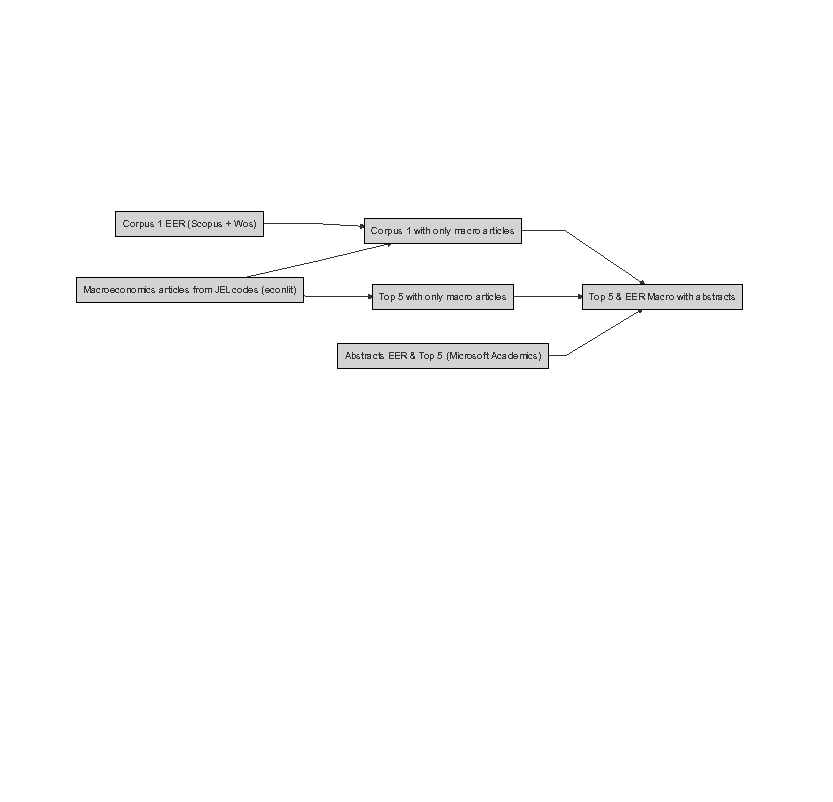
\includegraphics[width=1\linewidth]{First_version_files/figure-latex/plot-diagram-corpus-1} 

}

\caption{Construction of Corpus 2}\label{fig:plot-diagram-corpus}
\end{figure}

\hypertarget{b.2.-variable-creation}{%
\subsubsection*{B.2. Variable creation}\label{b.2.-variable-creation}}
\addcontentsline{toc}{subsubsection}{B.2. Variable creation}

\hypertarget{author-affiliation}{%
\paragraph*{Authors' affiliation}\label{author-affiliation}}
\addcontentsline{toc}{paragraph}{Authors' affiliation}

Authors' affiliations information were extracted from WoS. However, the
affiliations are not per author, but instead per institutional
departments per paper. For example, in the case of an article with two
authors from the same department, the department (and institution or
country associated with it) is only counted once. Similarly, a
single-authored article where the author has three affiliations can
result in one article having three affiliations. While in some cases we
can inferred the institutional affiliation for each author (e.g., one
institution, multiple authors), in others we cannot (e.g., two
institutions, three authors). For example, in an article with two
authors from Princeton and one author from Stanford, we only know that
the article was written by at least one author from Princeton and at
least one from Stanford, but not that the individual ratio was two
third.

We restructure the information in two ways.

First, for each article, we only kept one occurrence of each unique
institutions (university, research institutes\ldots) to avoid the
multiplication of observations resulting from the variety of departments
observed in some institutions. In other words, for each article, authors
are group by their institutional affiliation not by their department or
research team.

Second, and more importantly, for the purpose of our analysis, we mostly
looked at the share of papers authored by European-based and US-based
economists. While we do not have individual affiliation, we know with
certainty when a paper has only European authors, only American authors,
or a mix of the two. For this reason, while the share of institutions
within the corpus is only an estimation based on the occurrences of
affiliation, the information generated to identify US authored papers
and European authored paper is certain.

\hypertarget{network}{%
\subsubsection*{B.3. Bibliographic Coupling and Cluster
Detection}\label{network}}
\addcontentsline{toc}{subsubsection}{B.3. Bibliographic Coupling and
Cluster Detection}

A first way to identify potential differences between European and
American macroeconomics is to find articles written by Europeans and
published in European journals, resembling each others but dissimilar to
American articles. To do that, we used bibliographic coupling
techniques. In a bibliographic coupling network, a link is created
between two articles when they have one or more references in common.
The more references that two articles have in common, the stronger the
link. Bibliographic coupling is one way to measure how similar two
articles are in a corpus. To normalize and weight the link between two
articles, we used the refined bibliographic coupling strength of Shen et
al. (\protect\hyperlink{ref-shen2019}{2019}). This method normalized and
weight the strength between articles by taking into account two
important elements:

\begin{itemize}
\item
  the size of the bibliography of the two linked articles. It means that
  common references between two articles with long bibliography are
  weighted as less significant since the likeliness of potential common
  references is higher. Conversely, common references between two
  articles with a short bibliography is weighted as more significant.
\item
  the number of occurrences of each reference in the overall corpus.
  When a reference is shared between two articles, it is weighted as
  less significant if it is very common reference across the entire
  corpus and very significant if it is scarcely cited. The assumption is
  that a very rare common reference points to a higher content
  similarity between two articles than a highly cited reference.
\end{itemize}

For all macroeconomics articles published in the EER and in the Top 5,
we build the networks with 10-year overlapping windows. This results in
TO DO ALEX.

We used Leiden detection algorithm
(\protect\hyperlink{ref-traag2019}{Traag et al., 2019}) that optimize
the modularity on each network to identify groups of articles that are
similar to each others and dissimilar to the rest of the network. We use
a resolution of 1 with 1000 iterations. This results in TO DO ALEX
across all networks. Because networks have a lot of overlaps, many
clusters between two periods are composed of the same articles. To
identify these clusters that are very similar between two time windows,
we considered that \emph{(i)} if at least 55\% of the articles in a
community of the first time window where in the same cluster in the
second time window, and that \emph{(ii)} if the cluster was also
composed by at least 55\% of articles of the first time window,
\emph{then} it is the same cluster

Simply put, if two clusters share a high number of articles, and are
both mostly composed by these shared articles, they are considered the
same cluster.

This gives us TO DO ALEX, with TO DO ALEX that are at least 5\% of a
network at any given point and are stable enough to exists for at least
two time windows.

For each of these clusters, we computed the share of articles published
in the top 5 journals vs the EER, and the share of articles authored by
European vs American for the time window of the cluster We then
subtracted the share of articles published in the EER in the cluster
with the share of articles published in the EER on the same time period
of the cluster to identify over/under representation of the EER. We also
subtracted the relative share of European authors to American authors in
the cluster to the relative share of European authors to American on the
same time period of the cluster to identify over/under representation of
European authors in the cluster.

Finally, we plotted the clusters on a scatterplot to identify clusters
in which both European authors and the EER are over-represented.

\hypertarget{topic}{%
\subsubsection*{B.4. Topic Modelling}\label{topic}}
\addcontentsline{toc}{subsubsection}{B.4. Topic Modelling}

\hypertarget{preprocessing}{%
\paragraph*{Preprocessing}\label{preprocessing}}
\addcontentsline{toc}{paragraph}{Preprocessing}

We have several steps to clean our texts before running our topic
models:

\begin{enumerate}
\def\labelenumi{\arabic{enumi}.}
\tightlist
\item
  Once we have our corpus, we merge titles and abstracts together for
  all EER and Top 5 articles.
\item
  We use the \emph{tidytext} and \emph{tokenizers} R packages to
  `tokenise' the resulting texts (when there is no abstract, only the
  title if thus tokenise)?\footnote{See Silge J, Robinson D (2016).
    ``tidytext: Text Mining and Analysis Using Tidy Data Principles in
    R.'' \emph{JOSS}, \emph{1}(3) and Lincoln A. Mullen et al., ``Fast,
    Consistent Tokenization of Natural Language Text,'' Journal of Open
    Source Software 3, no.23 (2018): 655.} Tokenisation is the process
  of transforming human-readable text into machine readable objects.
  Here, the text is split in unique words (unigrams), bigrams (pair of
  words) and trigrams. In other words, to each article is now associated
  a list of unigrams, bigrams and trigrams, some appearing several times
  in the same title + abstract.
\item
  Stop words are removed using the \emph{Snowball}
  dictionary.\footnote{See
    http://snowball.tartarus.org/algorithms/english/stop.txt.} We add to
  this dictionary some current verbs in abstract like ``demonstrate'',
  ``show'', ``explain''. Such verbs are likely to be randomly
  distributed in abstracts, but we want to limit the noise as much as
  possible.
\item
  We lemmatise the words using the \emph{textstem} package.\footnote{Rinker,
    T. W. (2018). textstem: Tools for stemming and lemmatizing text
    version 0.1.4. Buffalo, New York.} The lemmatisation is the process
  of grouping words together according to their ``lemma'' which depends
  on the context. For instance, different form of a verb are reduced to
  its infinitive form. The plural of nouns are reduced to the singular.
\end{enumerate}

\hypertarget{choosing-the-number-of-topics}{%
\paragraph*{Choosing the number of
topics}\label{choosing-the-number-of-topics}}
\addcontentsline{toc}{paragraph}{Choosing the number of topics}

We use the Correlated Topic Model (\protect\hyperlink{ref-blei2007}{Blei
and Lafferty, 2007}) method implemented in the \emph{STM} R
package.\footnote{Roberts ME, Stewart BM, Tingley D (2019). ``stm: An R
  Package for Structural Topic Models.'' \emph{Journal of Statistical
  Software}, \emph{91}(2), 1-40.}

From the list of words we have tokenised, cleaned and lemmatised, we
test different thresholds and choices by running different models:

\begin{itemize}
\tightlist
\item
  by exluding trigrams or not;
\item
  by removing the terms that are present in less than 0.5\% of the
  Corpus (17), 1\% (34) and 2\% (68);
\item
  by removing articles with less than 6 words or with less than 12
  words.\footnote{Here, only articles with no abstract are impacted.}
\end{itemize}

Crossing all these criteria, we thus have 12 different possible
combinations. For each of these 12 different combinations, we have run
topic models for different number of topics from 20 to 110 with a gap of
5. The chosen model integrates trigram, removes only terms that appear
in less than 0,5\% of the documents and keep all articles if they have
more than 6 words in their title + abstract. We choose to keep the model
with 55 topics.

We have chosen the criteria and the number of topics by comparing the
performance of the different models in terms of the FREX value
(\protect\hyperlink{ref-bischof2012}{Bischof and Airoldi, 2012}).


\end{document}
